%Copyright 2014 Jean-Philippe Eisenbarth
%This program is free software: you can 
%redistribute it and/or modify it under the terms of the GNU General Public 
%License as published by the Free Software Foundation, either version 3 of the 
%License, or (at your option) any later version.
%This program is distributed in the hope that it will be useful,but WITHOUT ANY 
%WARRANTY; without even the implied warranty of MERCHANTABILITY or FITNESS FOR A 
%PARTICULAR PURPOSE. See the GNU General Public License for more details.
%You should have received a copy of the GNU General Public License along with 
%this program.  If not, see <http://www.gnu.org/licenses/>.

%Based on the code of Yiannis Lazarides
%http://tex.stackexchange.com/questions/42602/software-requirements-specification-with-latex
%http://tex.stackexchange.com/users/963/yiannis-lazarides
%Also based on the template of Karl E. Wiegers
%http://www.se.rit.edu/~emad/teaching/slides/srs_template_sep14.pdf
%http://karlwiegers.com
\documentclass{scrreprt}
\usepackage{listings}
\usepackage{underscore}
\usepackage[bookmarks=true]{hyperref}
\usepackage[utf8]{inputenc}
\usepackage[english]{babel}
\usepackage{CJKutf8}
\usepackage{graphicx}


\hypersetup{
    bookmarks=false,    % show bookmarks bar?
    pdftitle={Beverage Recognition System Requirement Specification},    % title
    pdfauthor={Jean-Philippe Eisenbarth},                     % author
    pdfsubject={TeX and LaTeX},                        % subject of the document
    pdfkeywords={TeX, LaTeX, graphics, images}, % list of keywords
    colorlinks=true,       % false: boxed links; true: colored links
    linkcolor=blue,       % color of internal links
    citecolor=black,       % color of links to bibliography
    filecolor=black,        % color of file links
    urlcolor=purple,        % color of external links
    linktoc=page            % only page is linked
}%
\def\myversion{1.0 }
\date{}
%\title
\usepackage{hyperref}
\begin{document}
\begin{CJK}{UTF8}{bkai}
\begin{flushright}
    \rule{16cm}{5pt}\vskip1cm
    \begin{bfseries}
        \Huge{Beverage Recognition System\\ SPECIFICATION}\\
        \vspace{1.9cm}
        for\\
        \vspace{1.9cm}
        Final Project\\
        \vspace{1.9cm}
        \LARGE{Version \myversion approved}\\
        \vspace{1.9cm}
        Prepared by Group4\\
        \vspace{1.9cm}
        \today\\
    \end{bfseries}
\end{flushright}

\tableofcontents

\chapter{Introduction}

\section{Purpose}
\underline{系統目標}
\begin{itemize}
\item[-] 提供通過圖片即時識別飲料並展示其詳細信息的系統
\item[-] 使用者可以通過上傳飲料圖片來了解此款飲料的配方、過敏原、營養成分以及飲料是否獲得認證。
\end{itemize}

\noindent \underline{系統範圍}

\begin{itemize}
\item[-] 接收使用者上傳圖片並顯示結果的網頁前端
\item[-] 對圖片進行識別並回傳結果的後端
\end{itemize}


\section{Intended Audience and Reading Suggestions}
本需求規格書用於提供給此專案之開發者以及測試者作為參考,包含有系統概述,功能定義說明,環境需求,使用者界面及操作說明,functional requirements以及nonfunctional requirements等\\
開發者在閱讀系統概述後應先從functional requirements開始著手設計系統
測試者應首先閱讀操作說明後再行測試

\section{Project Scope}
系統包含了提供給使用者上傳所要識別的飲料的網頁以及用於識別飲料並回傳飲料資訊的程式,旨在提供使用者對於飲料資訊更加快捷方便的查詢途徑


\chapter{Overall Description}

\section{Product Perspective}
本系統為一套獨立的系統,分為網頁程式與圖像識別程式兩個部分,如Figure 2.1所示

\begin{figure}[ht]
\begin{center}
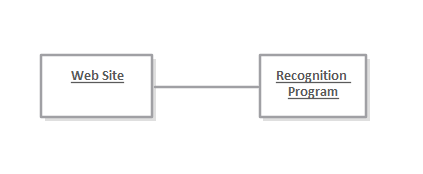
\includegraphics[width=8cm]{diagram1.png}
\end{center}
\caption{system simple diagram}
\label{fig:1}
\end{figure}

\section{Product Functions}
網頁接收到使用者上傳的圖像後,會將圖像傳至識別程式,由識別程式對飲料種類進行識別後,再回傳結果至網頁端,系統之dataflow diagram如Figure 2.2所示
\begin{figure}[ht]
\begin{center}
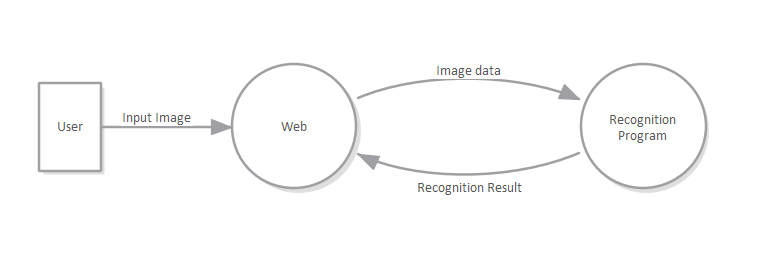
\includegraphics[width=14cm]{diagram2.png}
\end{center}
\caption{dataflow diagram}
\label{fig:1}
\end{figure}


\section{User Classes and Characteristics}
系統主要面向為經常使用手機和平板電腦進行上網查詢資料,較為注重飲食健康,或對某些飲料的配方成分會產生過敏反應的使用者對象

\section{Operating Environment}
服務器端:帶有Unix-like / Windows7及以上作業系統,可正常運作tensorflow程式之設備\\
使用者:能夠正常瀏覽網頁即可

\section{Design and Implementation Constraints}
\begin{itemize}
\item[-] 由於飲料品種資料蒐集的時間限制,系統只能支援識別市面上的一部分飲料
\item[-] 由於現有技術的限制,系統識別結果無法100\%準確
\end{itemize}

\section{Assumptions and Dependencies}
假設
\begin{itemize}
\item[-] 使用者上傳並非包含飲料的圖片
\item[-] 使用者上傳圖片過程中失敗
\end{itemize}
外部依賴
\begin{itemize}
\item[-] 深度學習套件
\item[-] 服務器與使用者需要有正常穩定的網路環境
\end{itemize}

\chapter{External Interface Requirements}

\section{User Interfaces}
使用者網頁介面需要:
\begin{itemize}
\item [1)]  可以選擇並且上傳待識別圖片的按鈕
\item [2)]  用於飲料詳細資訊的區塊
\end{itemize}
初始介面如Figure 3.1所示,系統需要在使用者上傳圖片,待識別程式識別成功並回傳結果後,在區塊內顯示識別結果之飲料的詳細資訊,如Figure 3.2所示

\begin{figure}[ht]
\begin{center}
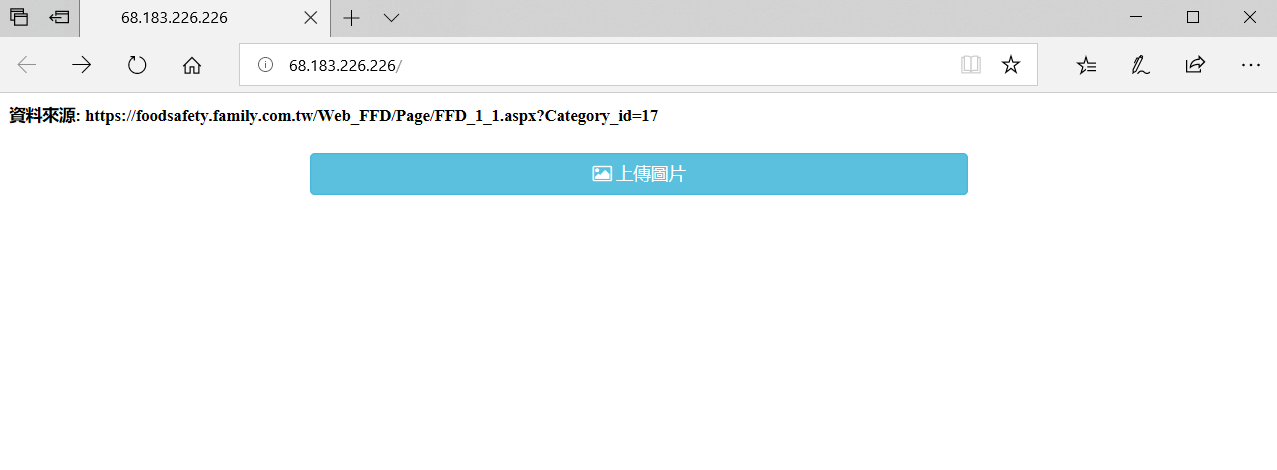
\includegraphics[width=14cm]{userinterface1.png}
\end{center}
\caption{User interface: before uploading image}
\label{fig:1}
\end{figure}

\begin{figure}[h]
\begin{center}
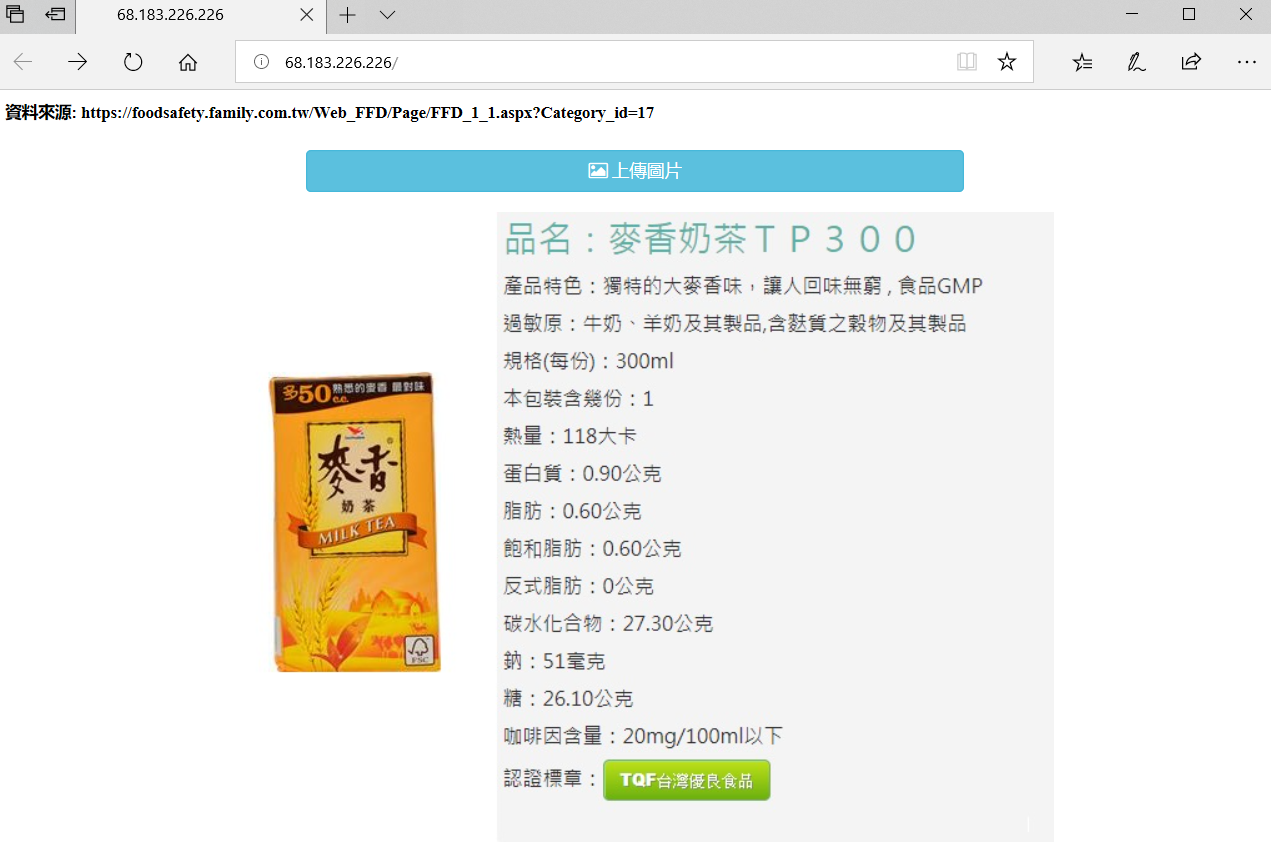
\includegraphics[width=14cm,height=10cm]{userinterface2.png}
\end{center}
\caption{User interface: show recognition result}
\label{fig:1}
\end{figure}

\section{Hardware Interfaces}
系統無需額外硬體組件
\section{Software Interfaces}
\begin{itemize}
\item[-] 在識別程式中使用OpenCV以三維矩陣的方式讀取外部圖像資料
\item[-] 本系統將會應用Tensorflow之深度學習框架,以及Keras模塊之API
\end{itemize}


\chapter{System Features}

\section{Description and Priority}
由於本系統是用於識別並顯示飲料資訊的系統,所以是否能正確識別出使用者給出的飲料較為重要,所以對於識別的準確度,本系統將放在最高優先級,其次是飲料資訊的詳細程度,其他的輔助項目將視需求會再陸續添加

\section{Stimulus/Response Sequences}
Use case 1: 
\begin{itemize}
\item [1)]  使用者進入網頁
\item [2)]  網頁顯示使用者介面
\item [3)]  點選 "上傳圖片" 按鈕,上傳所飲料圖片
\item [4)]	網頁顯示飲料之詳細資訊
\end{itemize}

Use case 2: 
\begin{itemize}
\item [1)]  使用者進入網頁
\item [2)]  網頁顯示使用者介面
\item [3)]  點選 "上傳圖片" 按鈕,上傳不包含飲料的圖片
\item [4)]	網頁顯示錯誤的飲料資訊
\end{itemize}

\section{Functional Requirements}
\begin{center}
\begin{tabular}{|l|c|r|}\hline
REQ1 & 圖片上傳\\ \hline
說明 & 提供使用者上傳待識別飲料圖片的功能\\ \hline
輸入 & 由使用者點選功能選項觸發\\ \hline
處理 & 將所選圖片傳至識別程式\\ \hline
輸出 & 網頁顯示上傳中之加載圖標\\ \hline
\end{tabular}
\end{center}

\begin{center}
\begin{tabular}{|l|c|r|}\hline
REQ2 & 飲料識別\\ \hline
說明 & 提供識別飲料並傳回結果的功能\\ \hline
輸入 & 識別程式接到使用者上傳的圖片後觸發\\ \hline
處理 & 識別圖中飲料並回傳識別結果\\ \hline
輸出 & 飲料種類\\ \hline
\end{tabular}
\end{center}

\begin{center}
\begin{tabular}{|l|c|r|}\hline
REQ3 & 飲料資訊顯示\\ \hline
說明 & 提供識別結果所示飲料的詳細資訊\\ \hline
輸入 & 接到飲料識別程式所傳回識別結果後觸發\\ \hline
處理 & 讀取識別結果所示飲料的詳細資訊\\ \hline
輸出 & 網頁顯示識別結果所示飲料之詳細資訊\\ \hline
\end{tabular}
\end{center}


\chapter{Other Nonfunctional Requirements}

\section{Performance Requirements}
識別準確度:
\begin{itemize}
\item[-] 由於本系統是用於提高使用者查詢飲料資訊效率的即時識別系統,所以對於飲料種類的單次識別應具有80\%以上的準確率
\end{itemize}
識別速度:
\begin{itemize}
\item[-] 由於本系統旨在提高使用者查詢飲料資訊效率,所以對於飲料種類的單次識別時間應控制在5s以內
\end{itemize}
可移植性:
\begin{itemize}
\item[-] 系統應在Unix-like作業系統與Windows作業系統上進行移植後可以正常運作
\end{itemize}
可測性:
\begin{itemize}
\item[-] 系統提供的功能均可以進行測試,以確保系統運作時的正確性
\end{itemize}
可維護性:
\begin{itemize}
\item[-] 系統提供的功能在建構時應加以模組化,以便後期易於維護以及功能易於增加或縮減
\end{itemize}
穩定性:
\begin{itemize}
\item[-] 本系統應具有較高的穩定性,能在99\%的時間內正常運作而不需要重啟系統
\end{itemize}


\end{CJK}
\end{document}
